%*********************************************************************************
\subsection{Simulation Experiment}\label{sub:sa_application_simulation_experiment}
%*********************************************************************************

The simulation experiment for global sensitivity analysis on the \gls[hyper=false]{trace} model of \gls[hyper=false]{feba} was carried out in two steps.
\marginpar{Screening analysis}
The first step was aimed at screening out any possible noninfluential parameters with relatively few code runs using several screening methods, i.e., the two variants of the Morris screening method (the radial and the trajectory designs) and the Sobol'-Saltelli method; with the latter only the total-effect indices were estimated, in line with the factor fixing objective.

The second step of the analysis consisted of variance decomposition through the estimation of the Sobol' indices on the reduced number of parameters.
\marginpar{Variance decomposition}
This was a more detailed analysis where the contribution of each input parameter variation to a particular output variance was quantified.
Since the number of code runs is directly proportional to the number of input parameters, 
the screening procedure done in the first step allowed us to reduce the size of the problem and to generate a larger sample for a fewer code runs\footnote{Note that the total duration of the transient is set to be $600 \ [s]$ and each TRACE run required between $\sim 400 - 600 \ [CPUs]$, where $[CPUs] = $ ``Central Processing Unit seconds''}.
A larger sample, in turn, led to a more precise Sobol' indices estimates.
The experimental design matrix used to carry out the estimation was generated using a Sobol' quasi-random sequence generator \cite{Joe2008}.

Different types of \glspl[hyper=false]{qoi} were investigated for this simulation experiment.
\marginpar{Quantities of Interest}
The application of the Morris method to the TRACE model of the FEBA facility to rank the parameter importance was already demonstrated in \cite{Wicaksono2014} using the time-averaged temperature as QoI, 
which is defined as
\begin{equation}
	\bar{T} = \frac{\int T(t) dt}{\int dt}
\label{eq:qoi_time_averaged_temperature}
\end{equation}
where the integration of the pointwise time-dependent reflood curve was approximated using the trapezoidal rule over the duration of the transient.
The time-averaged temperature was selected as the simplest possible scalar \gls[hyper=false]{qoi} to capture the overall variation of the temperature transient 
since it was previously shown that a high maximum cladding temperature as \gls[hyper=false]{qoi} would not necessarily imply a delayed time of quenching, and vice versa \cite{Wicaksono2014}. 
To further investigate these aspects, the maximum cladding temperature and the quench time have also been considered as \glspl[hyper=false]{qoi} in this study.

To represent better the notion of functional variation, \gls[hyper=false]{fda}-based techniques were applied to derive a new set of \glspl[hyper=false]{qoi}.
\marginpar{FDA-based Quantities of Interest}
All the steps required in the application of \gls[hyper=false]{fda} were already demonstrated in the context of the reflood simulation output in \cite{Wicaksono2014a}.
All the required computations related to \gls[hyper=false]{fda} were done with the \texttt{R} programming language \cite{RCT2017} using the \texttt{fda} package \cite{Ramsay2014}.
The application of \gls[hyper=false]{fda} resulted in a set of common \glspl[hyper=false]{fpc} and a set of realization-specific \gls[hyper=false]{fpc} scores.
The scores were therefore used as the \gls[hyper=false]{qoi} for the Sobol' indices estimation
and compared to the indices obtained from the more conventional \glspl[hyper=false]{qoi} for the reflood transient.

Finally, to give a measure of the uncertainty in all indices estimated by the Sobol'-Saltelli method, 
the $95$\% percentile \gls[hyper=false]{ci} were constructed using the bootstrap technique (see \cite{Efron1986} and for detail).
The flowchart of the simulation experiment for the analysis is illustrated and summarized in Fig.~\ref{fig:sensitivity_flowchart}.

\begin{sidewaysfigure}
	\centering
	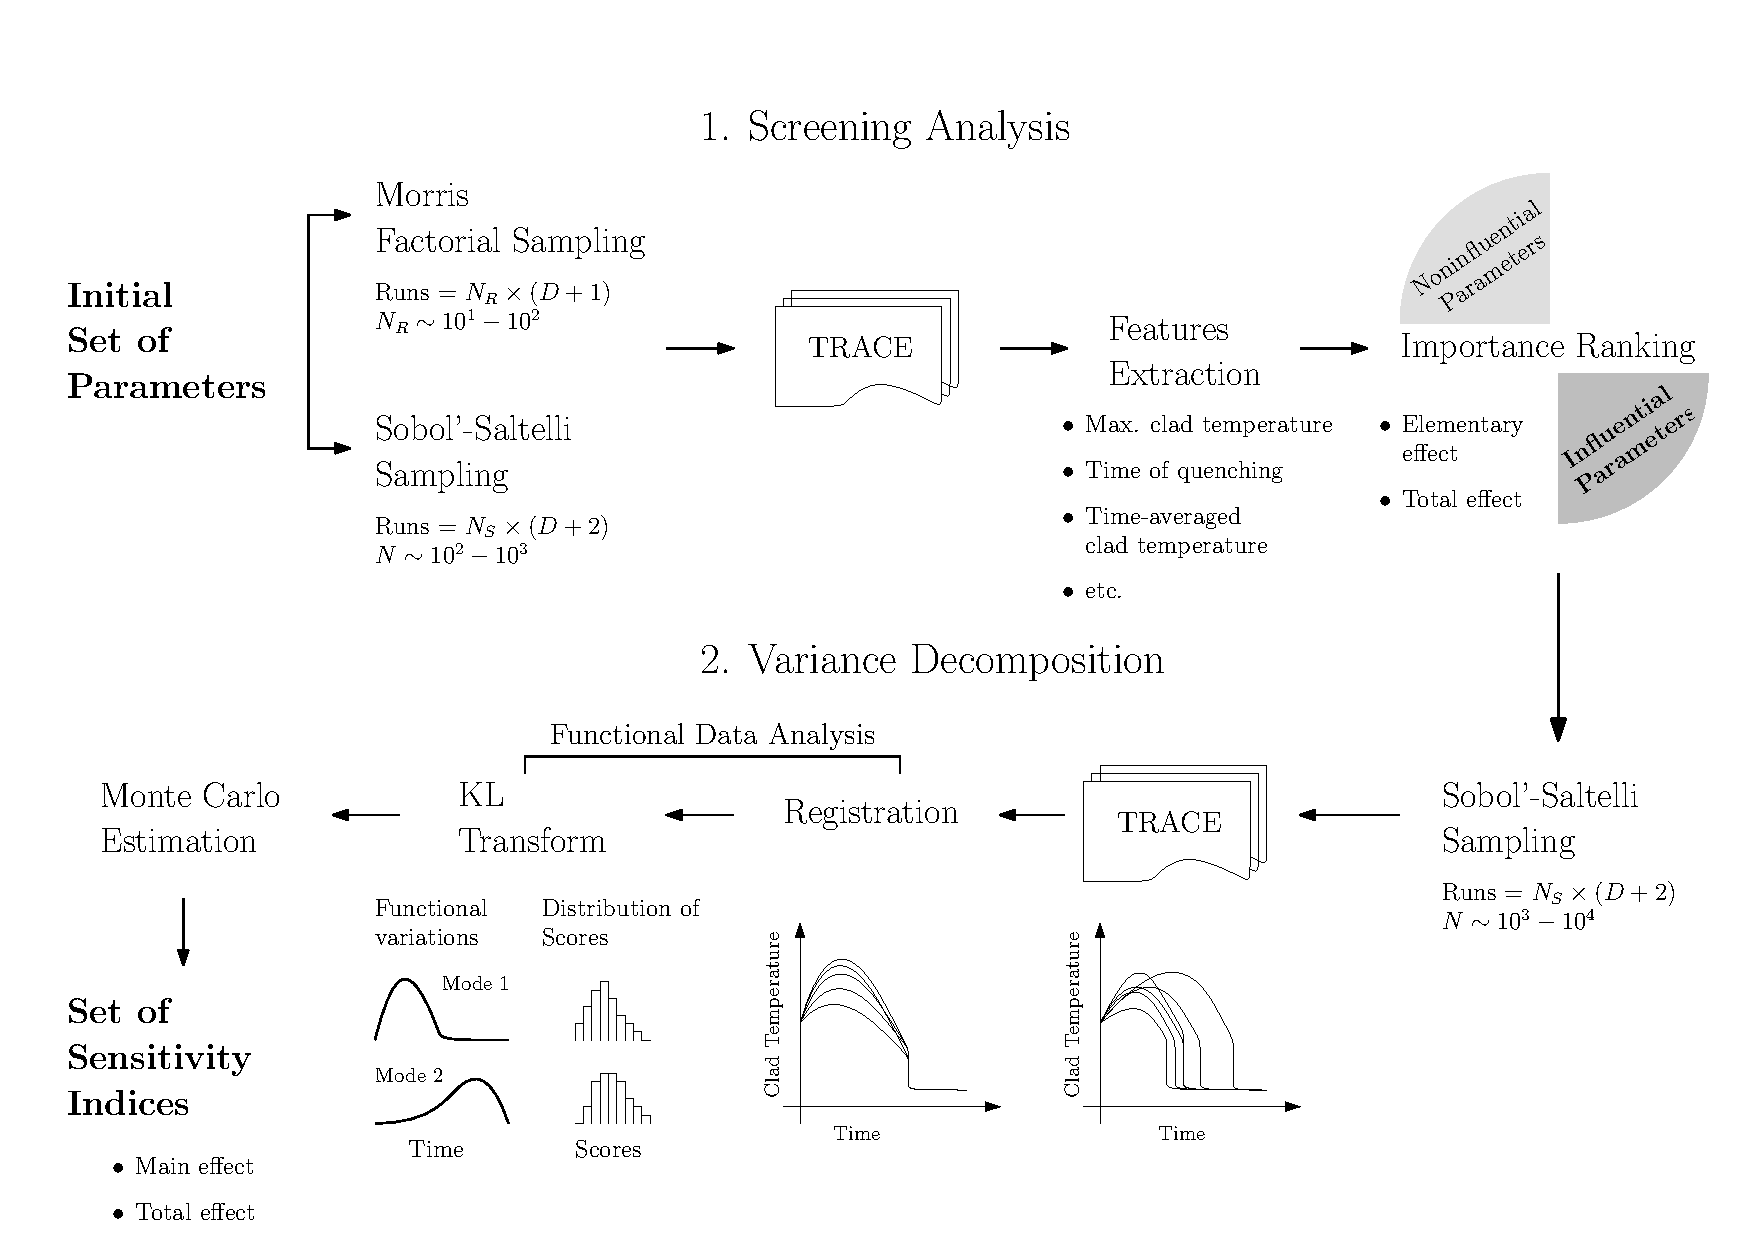
\includegraphics[width=0.85\textwidth]{../figures/chapter3/figures/simulation_experiment}
	\caption[Flowchart for the implemented sensitivity analysis methodology applied to the TRACE model of the FEBA facility]{Flowchart for the implemented sensitivity analysis methodology applied to the \gls[hyper=false]{trace} model of the \gls[hyper=false]{feba} facility.}
	\label{fig:sensitivity_flowchart}
\end{sidewaysfigure}

